Ultimo e più importante passaggio dell'algoritmo: dato il dataset prodotto in output dalla fase precedente,
viene eseguita una ricerca di pattern di co-movimento utilizzando i principi del \textit{Colossal Trajectory Mining}.

Il punto di partenza per questo step è Carpenter~\cite{DBLP:conf/kdd/PanCTYZ03}: tale algoritmo ricerca
insiemi di feature frequenti generando una versione trasposta del dataset originale, chiamata \textit{TT} un albero, chiamato \textit{row enumeration tree} avente nei nodi tutti i possibili set di transazioni;
successivamente questo viene esplorato utilizzando una ricerca \textit{depth-first}.
In~\cref{fig:chap-3:carpenter} viene presentato un esempio di quanto detto sopra.

\begin{figure}
  \centering
  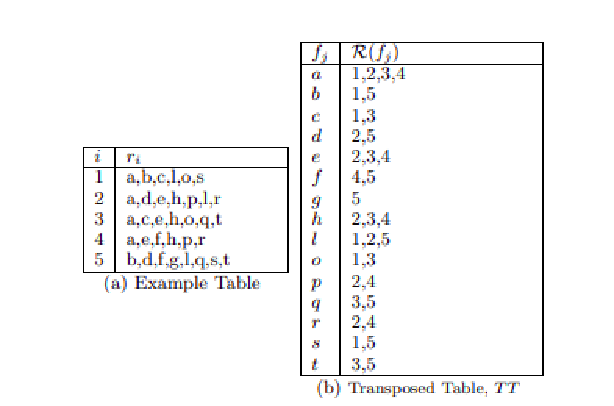
\includegraphics[scale=.6]{/sec-3/CarpenterTableSet.pdf}
  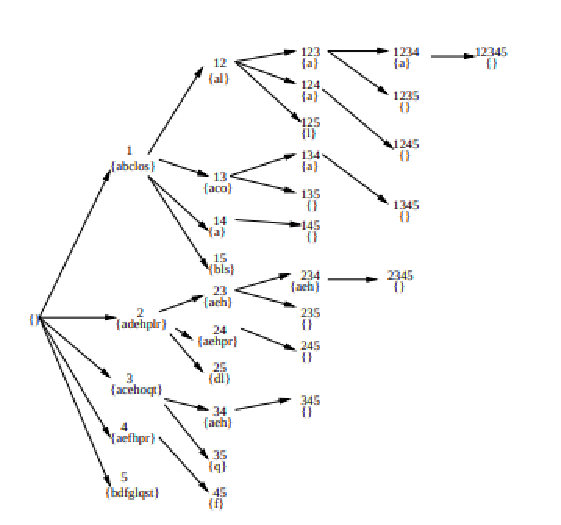
\includegraphics[scale=.6]{/sec-3/CarpenterEnumerationTree.pdf}
  \caption{Esempio di \textit{TT} e \textit{Row Enumeration Tree},Fonte:~\url{https://which.souce?}}%
  \label{fig:chap-3:carpenter}
\end{figure}

Carpenter per definizione ricerca pattern chiusi
